\documentclass[9pt, oneside]{article}   	% use "amsart" instead of "article" for AMSLaTeX format
\usepackage[left=2cm, right=2cm, top=3cm]{geometry}
\usepackage{cite}
\usepackage[english]{babel}
\usepackage{geometry}                		% See geometry.pdf to learn the layout options. There are lots.
\geometry{letterpaper}                   		% ... or a4paper or a5paper or ... 
\usepackage{graphicx,kantlipsum,setspace}
\usepackage{caption}			% Use pdf, png, jpg, or eps§ with pdflatex; use eps in DVI mode
\captionsetup[table]{font={stretch=1.15}}     %% change 1.2 as you like
\captionsetup[figure]{font={stretch=1.15}} 
\graphicspath{ {images/} }		% TeX will automatically convert eps --> pdf in pdflatex
\PassOptionsToPackage{hyphens}{url}\usepackage{hyperref}
\renewcommand{\UrlFont}{\small\tt}
\usepackage[euler]{textgreek}
\usepackage{verbatim}						
\usepackage{titlesec}
\titlelabel{\thetitle.\quad}
\usepackage{amssymb}
\linespread{1.15}
\usepackage{gensymb}
\usepackage{textcomp}
\usepackage{setspace}
\usepackage[symbol]{footmisc}
\usepackage[version=4]{mhchem}
\usepackage{multicol}
\setlength\columnsep{20pt}
\usepackage{wrapfig}
\setlength{\parindent}{1cm} % Default is 15pt.


% 2 is subsection, 3 is subsubsection
\setcounter{tocdepth}{3}

\begin{document}
\newpage


\begin{center}
\Large{\textbf{Estimating Filecoin Electricity Consumption from On-Chain Proofs}}
\vspace{1 cm}

\normalsize{}
Alan Ransil

Protocol Labs

alan@protocol.ai

\vspace{1 cm}
Model Version 1.0.1

Updated \today

\vspace{1 cm}
\Large{\textbf{Abstract}}

\end{center}

\noindent Emissions due to electricity consumption are a major component of the environmental impact of Web3 technologies. These emissions are challenging to estimate due to the distributed and permissionless nature of cryptocurrency networks. In this work we examine the electricity use of Filecoin, the world’s largest decentralized data storage network, leveraging architectural features that aid analysis of electricity use. Firstly, storage providers (SPs) contributing to the network do so by providing non-fungible data storage services. The blockchain thus contains a precise record of computing resources contributed by each SP at every point in time, facilitating both granular and network-wide electricity use estimates. Secondly, the computing resources contributed to the network are extremely similar to those of typical data centers, allowing us to bring literature findings on data center energy use to bear. We collect data from sources including questionnaires, interviews with SPs, benchmarks, and hardware specifications to estimate and bound Filecoin electricity consumption. The model results are comparable to estimates for average data centers, with Filecoin consuming 0.62\% of global data center electricity use estimated in 2020 while storing 0.77\% of global data storage capacity estimated in that same year. The resulting model is presented as a public dashboard allowing evaluation of energy consumption for both individual SPs and the network as a whole based on storage proofs from the Filecoin blockchain. This work forms the basis for a granular and publicly verifiable understanding of interactions between the Filecoin network and local power systems.



\begin{multicols}{2}
\setlength{\parskip}{0.1\baselineskip} %Controls vertical space between paragraphs, can re-set line by line
\section{Model Design (v1.0.1)}

Filecoin, the world’s largest distributed storage network, allows Storage Providers (SPs) to contribute storage capacity in exchange for a higher chance of winning the block reward. In order to ensure that replicated data is being stored over time, SPs must submit Proofs of Storage (also called Proofs of Spacetime, or PoSts) to the Filecon blockchain every 24 hour period. These proofs provide a cryptographic guarantee that data is continuing to be stored, and rely on a one-time setup process known as Sealing (also called Proof of Replication, or PoRep). During Sealing, Succinct Non-interactive Arguments of Knowledge (SNARKs) are generated for a data sector and recorded on the blockchain. This then enables subsequent PoSt proofs to be validated.

For our purposes, namely making a first attempt to estimate the energy use of Filecoin based on on-chain data, there are three relevant aspects of SP activity. Firstly, the process of Sealing a sector is energy intensive. According to benchmarks, this process generally takes about 5-6 hours of compute time in order to seal a 32 GiB sector. Secondly, the energy used to store data over time is relevant to overall energy use estimates. Thirdly, the overhead energy used to perform functions such as cooling and power conversion substantially affects estimates.

A sector needs to be sealed only once but its data must be stored over time, implying an ongoing energy use. Dimensional analysis thus implies the following equation:

\[
P = ( A * SR + B * Cap) * PUE
 \tag{Equation 1}
 \label{estimateEq}
\]

For an entity (either the network as a whole or an individual SP):

\textbf{P (Electrical Power, Watts)} is the electricity use of the entity.

\textbf{A (Sealing Energy Constant, Wh/byte)} is the energy required to seal a sector.

\textbf{SR (Sealing Rate, bytes/hour)} is the rate at which new data is being sealed by that entity.

\textbf{B (Storage Energy Constant, W/byte)} is the electrical power required to store data.

\textbf{Cap (Raw Capacity, bytes)} is the amount of data stored by the entity.

\textbf{PUE (Power Usage Effectiveness, dimensionless)} is the Power Usage Effectiveness, which is the ratio of total electrical power consumed to that consumed by IT processes.

As the Sealing Rate and Raw Capacity can be determined using on-chain proofs, the remaining goal is to determine the upper bound, lower bound and estimated values of A, B and PUE.

\section{Aspects not considered by this model, and rationale (v1.0.1)}

In this model, we do not account for power used to generate PoSt proofs. This is because while generating PoRep requires producing 11 SNARK proofs corresponding to one sector, PoSt requires the equivalent of generating 1 SNARK proof corresponding to over 2,000 sectors. The ongoing requirement of PoSt proof generation is thus orders of magnitude smaller than the uncertainty in the power use estimates provided below.

We also do not account for the energy used to produce and validate blocks. This is because the Proof of Storage consensus mechanism used in Filecoin elects a leader and allocates the block reward using a verifiable randomness beacon. This process may be considered analogous to the energy-efficient proof of stake consensus mechanism, in which the probability of a block reward is proportional to sealed storage contributed to the network rather than staked tokens. Again, the energy used by this process is small compared to the components of energy use described above.

\section{Sealing Energy (v1.0.1)}

Data used to estimate the sealing energy came from three sources: (1) a survey sent to SPs asking about their sealing energy use, (2) detailed conversations with SPs in order to better understand their rig design and sealing energy use methodology, and (3) benchmark results combined with thermal design power ratings used to contextualize the data received from these sources. Datapoints from all three sources are shown in Figure 1 and Table 1.

Survey data was derived from the following questions:

\begin{enumerate}
\item Over the past 28 days, how much storage capacity have you added to the Filecoin network?
\item What is the peak power of your sealing hardware based on manufacturer’s specifications (including any GPU, CPU or other processor but not including power supply, hard drives, cooling, etc)?
\item What do you estimate is the average power use of your sealing hardware (ie. kWh/day) or equivalently, what is the average time per day it is running near full power? (ie. 20hours/day)
\end{enumerate}

Results in Wh/byte were calculated based on responses to these questions. 

The data reported from surveys spans several orders of magnitude. While some of the variation is due to differences in actual sealing efficiency due to rig design, the majority of this spread is attributed to methodological differences in survey responses.

\end{multicols}
\begin{center}
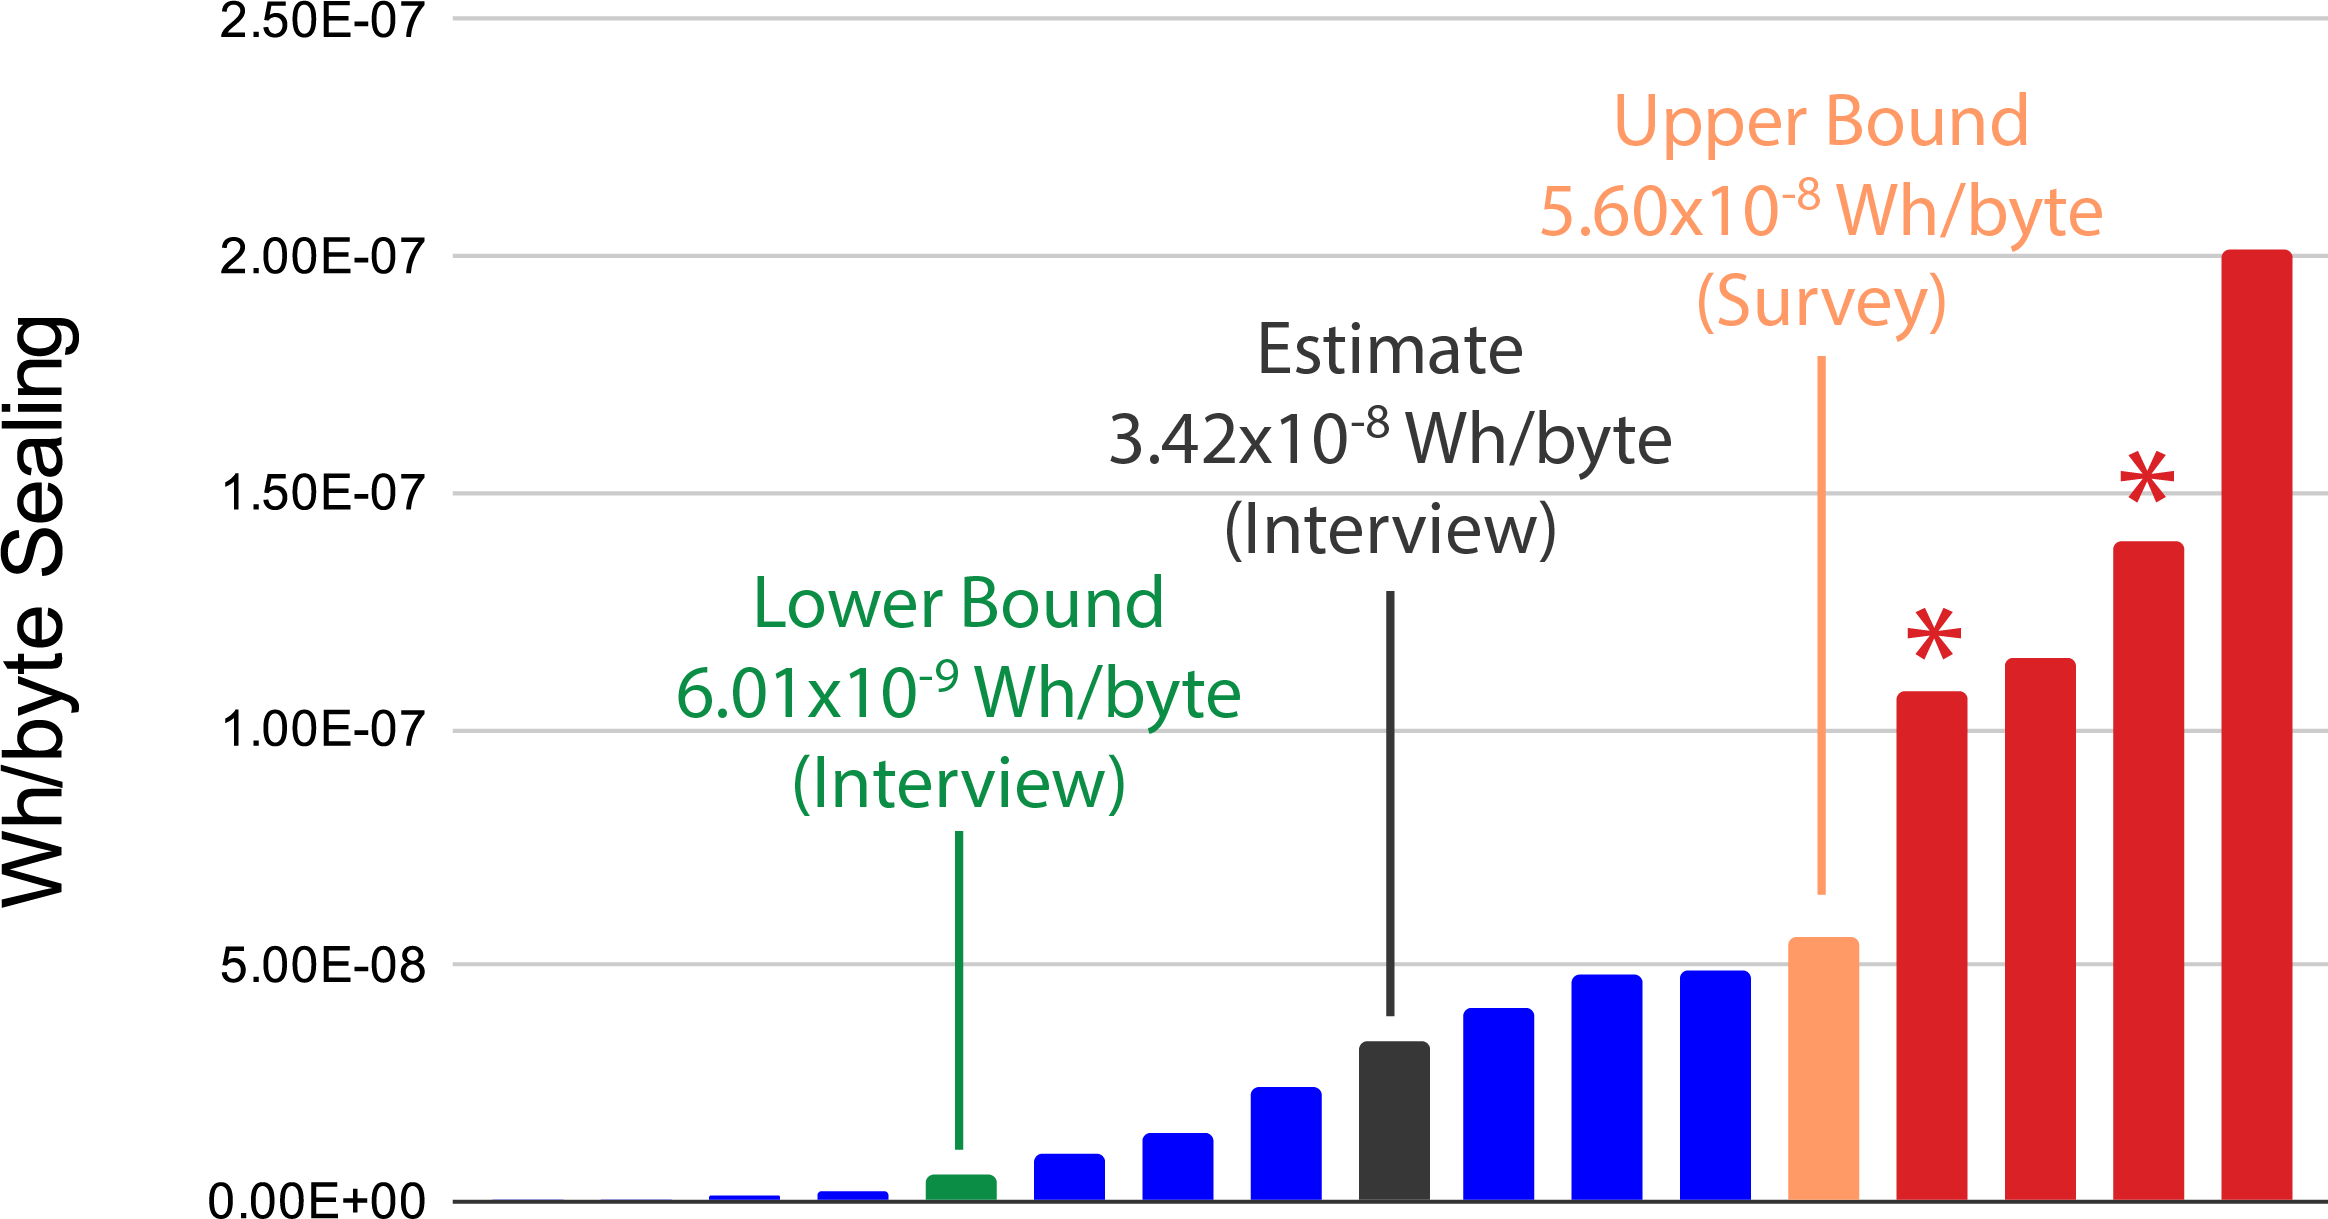
\includegraphics[width=.8\columnwidth]{20211023_SealingValues}
\begin{flushleft}
\captionof{figure}[Sealing Data]{Graph of datapoints used to estimate parameter A in \ref{estimateEq}, corresponding to the energy required to seal one byte of data. Values marked with an asterisk correspond to TDP calculation shown in tables 2 and 3.}
\label{sealingenergyfigure}
\end{flushleft}
\end{center}
\begin{multicols}{2}

\small
 \noindent \begin{tabular}{|| p{2cm} | p{2.5cm} | p{2.5cm} ||} 
 \hline
 \textbf{A (Wh/byte)} & \textbf{Source} & \textbf{Notes}\\
   \hline
 $2.8 \cdot 10^{-12}$ & Survey &  \\
  \hline
 $2.49\cdot 10^{-11}$ & Survey &  \\
   \hline
$1.27\cdot 10^{-9}$ & Survey &  \\
  \hline
$2.33\cdot 10^{-9}$ & Survey &  \\
  \hline
$6.01\cdot 10^{-9}$ & Interview & Lower Bound \\
  \hline
$1.03\cdot 10^{-8}$ & Survey &  \\
  \hline
$1.43\cdot 10^{-8}$ & Survey &  \\
  \hline
$2.44\cdot 10^{-8}$ & Survey &  \\
  \hline
$3.42\cdot 10^{-8}$ & Interview & Estimate \\
  \hline
$4.07\cdot 10^{-8}$ & Survey &  \\
  \hline
$4.80\cdot 10^{-8}$ & Survey &  \\
  \hline
$4.85\cdot 10^{-8}$ & Survey &  \\
  \hline
$5.60\cdot 10^{-8}$ & Survey & Upper Bound \\
  \hline
$1.08\cdot 10^{-7}$ & Benchmark time @ TDP (Table 2) & Unrealistically high \\
  \hline
$1.15\cdot 10^{-7}$ & Survey &  \\
  \hline
$1.40\cdot 10^{-7}$ & Benchmark time @ TDP (Table 2) & Unrealistically high \\
  \hline
$2.02\cdot 10^{-7}$ & Survey &  \\
  \hline
\end{tabular}
  \captionof{table}[Sealing Energy Data]{Values used to estimate parameter A in \ref{estimateEq}, corresponding to the energy required to seal 1 byte of data.}
\label{sealingEnergyTable}
\normalsize{}

In order to derive a narrower and more useful estimate, we examined both the upper and lower bounds of the spectrum. Firstly, the thermal design power was calculated by examining benchmark results for reference sealing machine architectures. The results are shown in Table 3, and marked with asterisks in Figure 1. As during alternate stages of sealing only the CPU or GPU is active, this is expected to be a significant overestimate of sealing energy. Survey values within this range, highlighted in red in Figure 1, are assumed to have been provided according to a Thermal Design Power (TDP) -equivalent methodology. An upper bound value of $5.60 \cdot 10^{-8}$ Wh/byte was chosen. This value is about half of the TDP, which we expect corresponds to the performance of a smaller, less optimized SP system.

The lower bound was determined through interviews with a larger, highly optimized SP. By parallelizing the sealing process across CPU threads, this SP is able to achieve a highly efficient process. A value of $6.01 \cdot 10^{-9}$ Wh/byte obtained from this SP was used as a lower bound. It is possible that some SPs are able to achieve more efficient processes. However, we are skeptical that the low range of reported survey values are possible and suspect that they are due to methodological error. Furthermore, we would prefer to overestimate energy use rather than underestimate.

\end{multicols}
\begin{center}
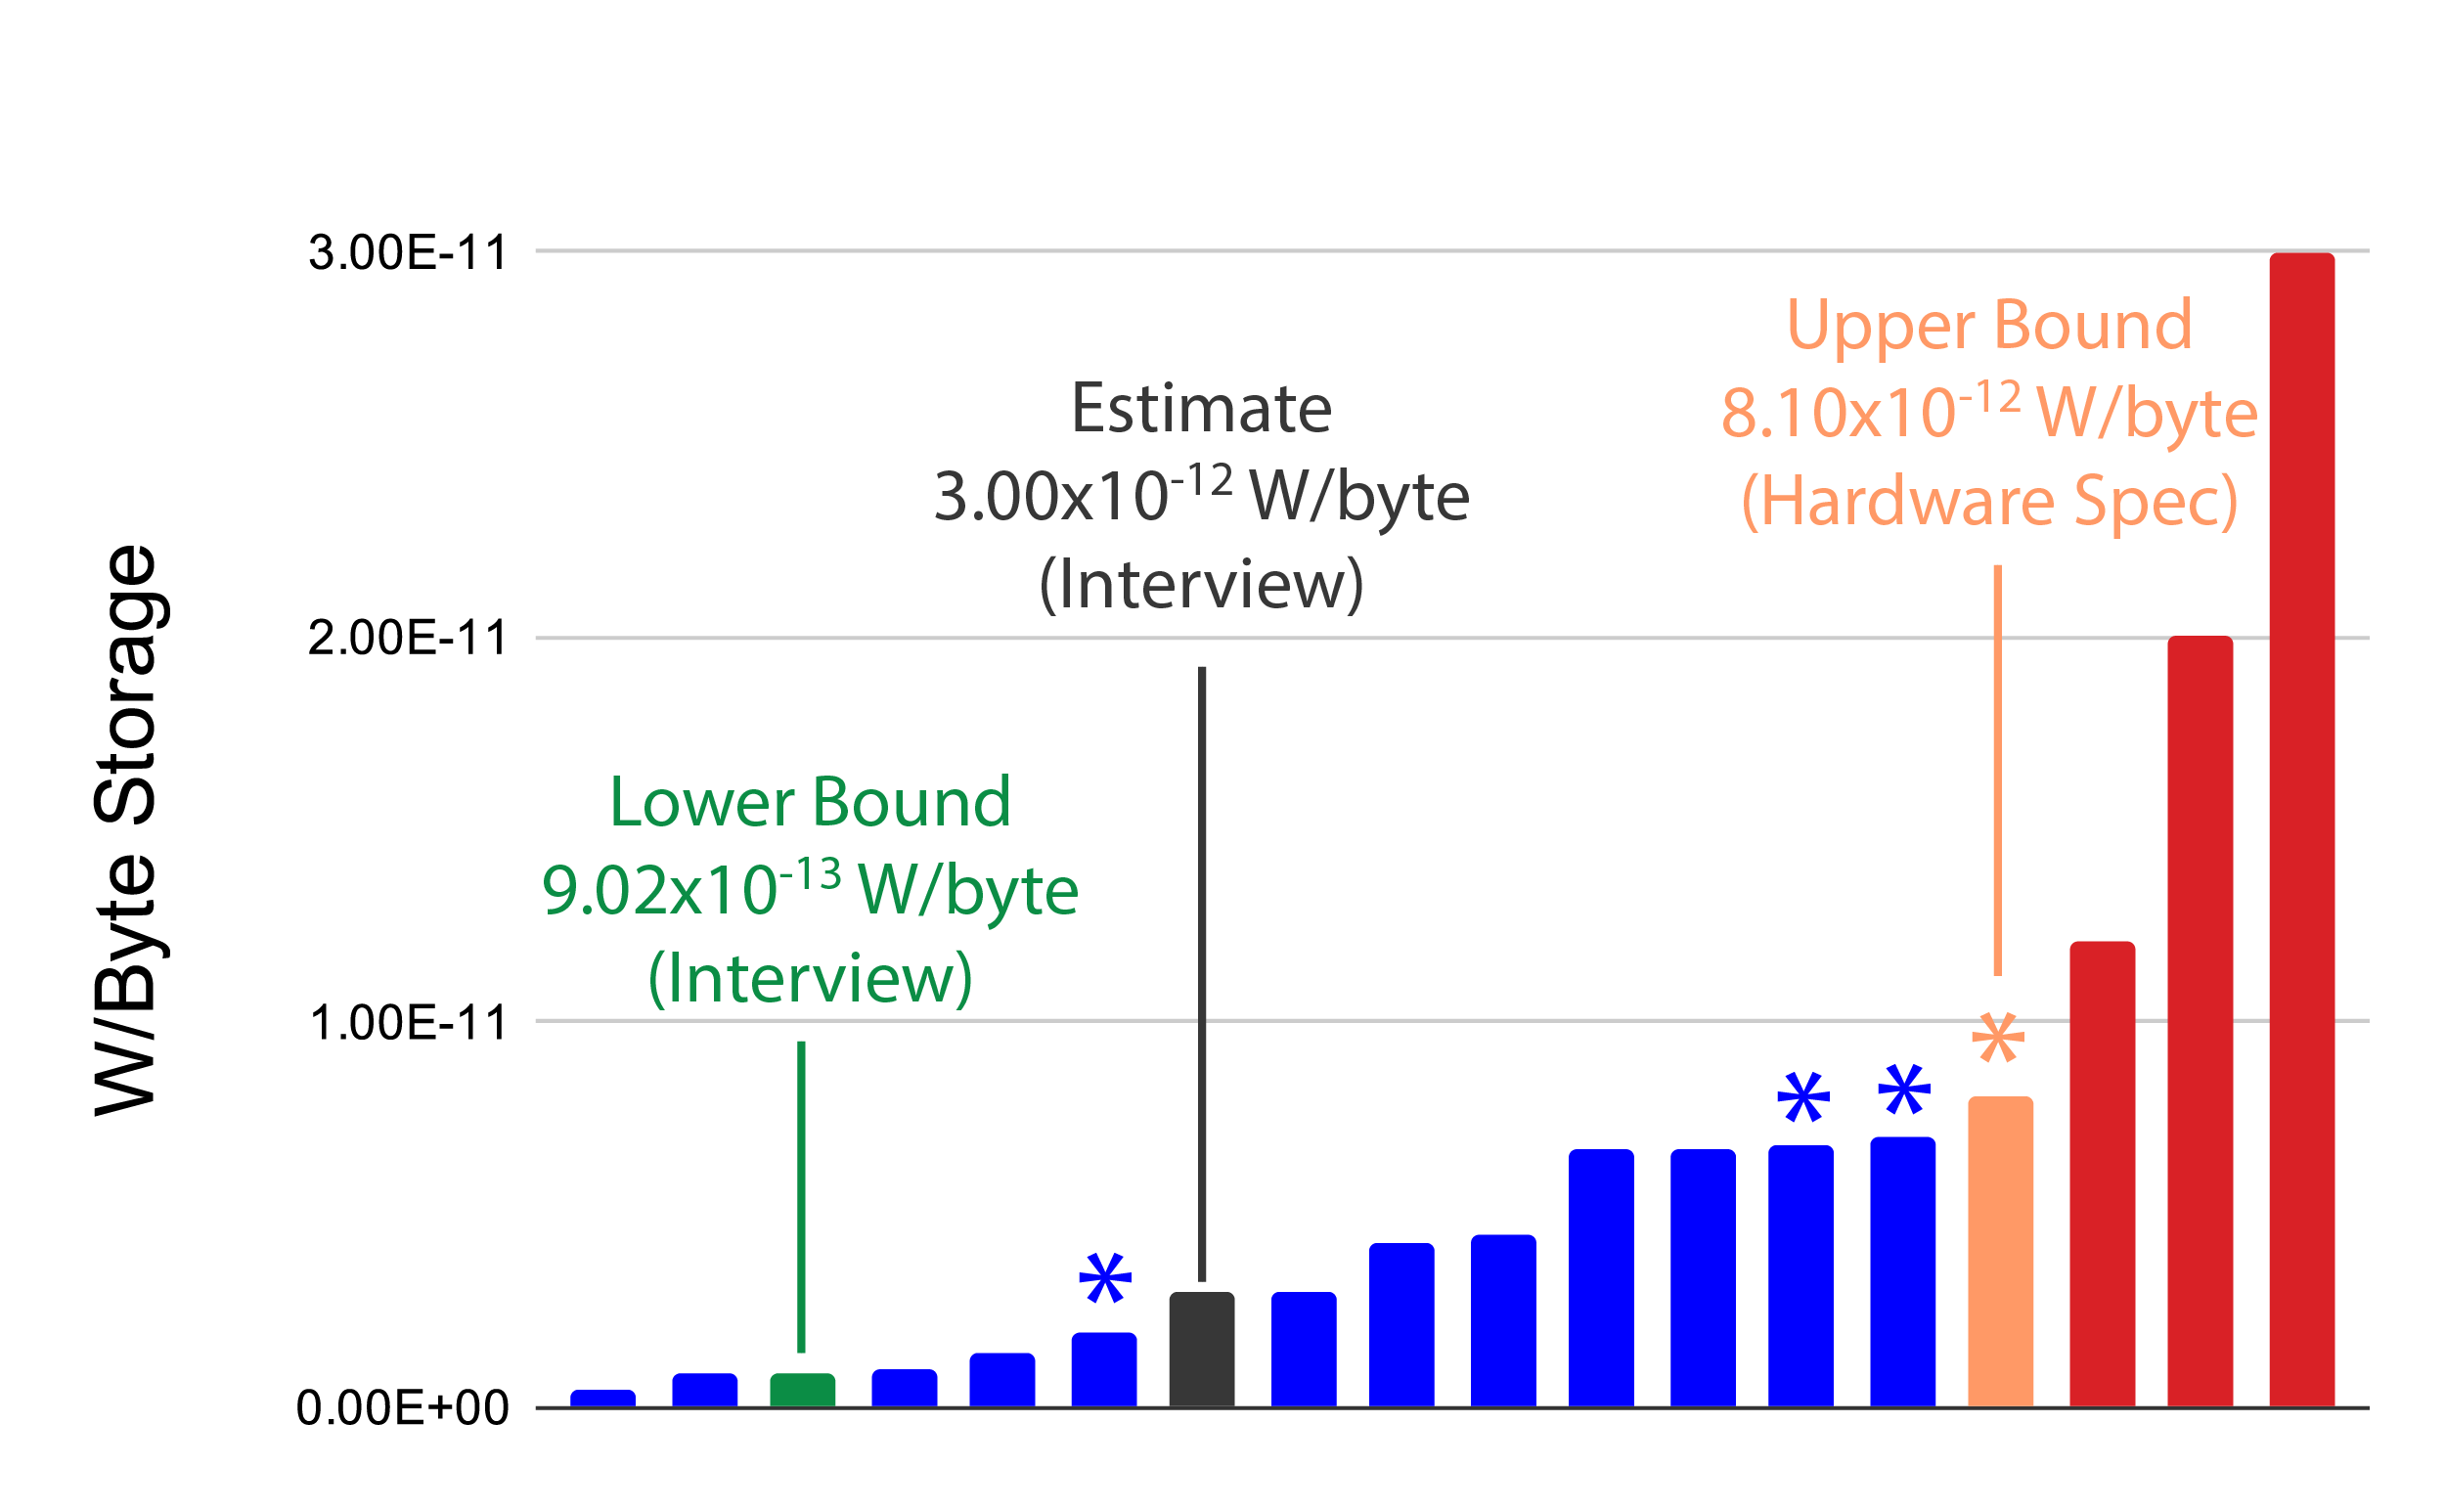
\includegraphics[width=.8\columnwidth]{20211023_StorageValues_withRefDrives}
\begin{flushleft}
\captionof{figure}[Storage Data]{Graph of data used to determine values for parameter B in \ref{estimateEq}, corresponding to the average electrical power needed to store one byte of data in the network. Bounds and estimate used are marked. Values marked with an asterisk are derived from spec sheets.}
\label{storageEnergyFigure}
\end{flushleft}
\end{center}
\begin{multicols}{2}

\small
 \noindent \begin{tabular}{|| p{2cm} | p{2.5cm} | p{2.5cm} ||} 
 \hline
 \textbf{B (W/byte)} & \textbf{Source} & \textbf{Notes}\\
   \hline
 $2.8 \cdot 10^{-12}$ & Survey &  \\
  \hline
$5.21\cdot 10^{-13}$ & Survey &  \\
\hline
$8.57\cdot 10^{-13}$ & Survey &  \\
\hline
$9.02\cdot 10^{-13}$ & Interview & Lower Bound \\
\hline
$1.03\cdot 10^{-12}$ & Survey &  \\
\hline
$1.42\cdot 10^{-12}$ & Survey &  \\
\hline
$1.90\cdot 10^{-12}$ & Survey &  \\
\hline
$3.00\cdot 10^{-12}$ & Interview & Estimate \\
\hline
$3.03\cdot 10^{-12}$ & Survey &  \\
\hline
$4.23\cdot 10^{-12}$ & Survey &  \\
\hline
$4.44\cdot 10^{-12}$ & Survey &  \\
\hline
$6.67\cdot 10^{-12}$ & Survey &  \\
\hline
$6.67\cdot 10^{-12}$ & Survey &  \\
\hline
$6.80\cdot 10^{-12}$ & WD 2019 (1) &  \\
\hline
$7.00\cdot 10^{-12}$ & Seagate 2016 &  \\
\hline
$8.10\cdot 10^{-12}$ & WD 2019 (2) &  \\
\hline
$1.21\cdot 10^{-11}$ & Survey &  \\
\hline
$2.00\cdot 10^{-11}$ & Survey &  \\
\hline
$3.00\cdot 10^{-11}$ & Survey & Not shown in figure (extremely high) \\
\hline
 \end{tabular}
  \captionof{table}[Sealing Energy Data]{Values used to estimate parameter B in \ref{estimateEq}, corresponding to the average electrical power needed to store one byte of data.}
\label{storageEnergyTable}
\normalsize{}

\indent{}

The estimated value was obtained from interviews with a mid-sized SP. This datapoint was chosen because this operation is expected to be representative of the median SP, and fell near the center of the distribution from survey data. It is likely that this is an overestimate of the energy required for sealing across the network as a whole, because most data is stored with larger and more optimized providers.

\section{Storage Energy (v1.0.1)}

Storage energy was estimated using (1) a survey sent to SPs, (2) detailed conversations with individual SPs in order to better understand their storage hardware and sources of variation, and (3) values from several hardware specification sheets.

Survey results were obtained by asking the following question:

\begin{enumerate}
\item What is the power consumption and capacity of a storage rack in your system? (example: 30kW per 4.5 PB rack)
\end{enumerate}

The resulting data was converted into a Wh/byte estimate.

Storage energy is susceptible to several large sources of variation. Firstly, many sectors may be stored on one hard drive, but the entire drive must be obtained and accessed when that sector is written or read which calls into question the assumption that sealing energy is directly proportional to the amount of data stored. Future work should develop alternative ways of modeling storage energy. Secondly, the energy efficiency of hard drives has improved rapidly over the past several years (continuing a decades-long trend). Thus, SPs with older hard drives may use dramatically more energy to store the same data. Third, hard drive configuration has a substantial impact on energy use. Large SPs with the ability to build large RAID arrays will frequently be able to keep drives idle, dramatically improving energy efficiency compared to smaller players who use fewer hard drives.

Survey data obtained shows a range of several orders of magnitude. On the high end, survey datapoints showing values significantly greater than the operating power use of 1 TB consumer hard drives (Table 5) were assumed to be unrealistically high and likely the result of methodological error. An operating power from a 1 TB 2019 hard drive was chosen as the upper bound. It is expected that this substantially overestimates energy use for the network as a whole, as most operators weighted by storage capacity will be larger data center operations making use of highly optimized disk arrays and utilizing newer, more energy efficient hardware.

The lower bound and estimate were taken to be values of storage energy derived from the same SPs as chosen in the sealing energy case. These SPs are large (lower bound) and mid-sized (estimate), with a high and moderate degree of optimization respectively. 

\section{Power Usage Effectiveness (v1.0.1)}

Power usage effectiveness (PUE) is a measure of the energy efficiency of a data center, and is given by:

\[
PUE = \frac{Power_{Total}}{Power_{IT}}
 \tag{Equation 2}
 \label{pueEq}
\]

Lower PUE values correspond to less overhead energy use such as cooling and power conversion losses, compared to the electrical load performing useful functions. Finding average PUE values of datacenters in a given region is a subject of debate. For our model, we used values from the literature as shown in Table 6. The lower bound corresponds to the estimated PUE of highly efficient hyperscale data centers, the estimate corresponds to an industry average, while the upper bound was taken to be that of ‘traditional’ data centers which are smaller and less optimized operations.



\end{multicols}
\vspace{1 cm}
\begin{center}
 \noindent \begin{tabular}{||  | p{3cm} | p{3cm} | p{4cm} | p{5cm} ||} 
 \hline
  & \textbf{PUE Value} & \textbf{Source} & \textbf{Notes}\\
   \hline
 Lower Bound & 1.18 & Masanet et al., 2020 & Hyperscale Data Centers\\
    \hline
 Estimate & 1.57 & 2021 Uptime Institute & Industry Average\\
    \hline
Upper Bound & 1.93 & Masanet et al., 2020 & Traditional Data Centers\\
   \hline
\end{tabular}
\begin{flushleft}
\captionof{figure}[PUE Data]{PUE values and sources for Filecoin network model.}
\label{pueTable}
\end{flushleft}
\end{center}
\begin{multicols}{2}


\end{multicols}
\end{document}  


